\section{Algorithm proposal}
This assignment propose an algorithm to solve the problem and will utilize dynamic programming techniques and inspiration from the divide and conquer pattern to solve it efficiently.
The optimal solution to the problem can be constructed of solutions to sub problems that could have been computed before, thus memorization can be used.
The optimal solution is found by either picking first or last card plus the optimal solution with rest of the cards where ronald picks first.


The following diagram illustrates a scenario of a given problem at the initial state.
\begin{figure}[H]
    \centering
    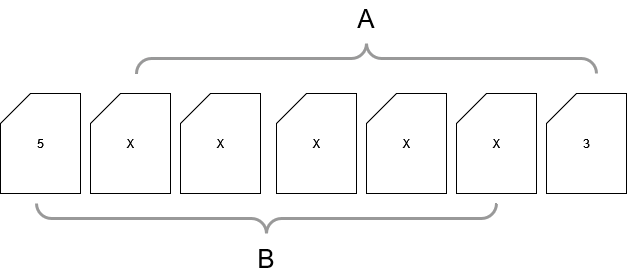
\includegraphics[width=0.6\textwidth]{images/diagram1.png}
    \caption{Diagram illustrating scenario of initial state of a problem}
    \label{fig:D1}
\end{figure}
The optimal solution is then: $\text{Max}\begin{cases}
    5 + \text{Best solution with cards in: }A \\
    3 + \text{Best solution with cards in: }B
\end{cases} $

To continue the example, the following diagram illustrates the scenario where 5 was picked and best solution with cards in A is then needed.
\begin{figure}[H]
    \centering
    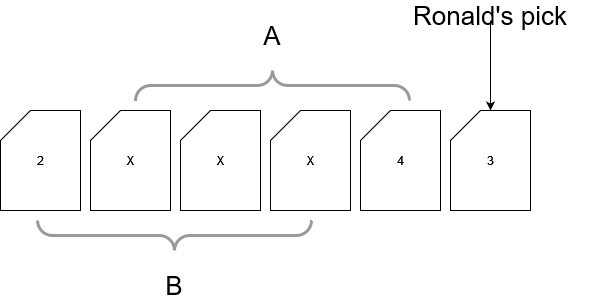
\includegraphics[width=0.6\textwidth]{images/diagram2.png}
    \caption{Diagram illustrating a scenario in which ronald picks next}
    \label{fig:D2}
\end{figure}

With Ronald's strategy being known, one card can be removed and the patterns as in figure \ref*{fig:D1} can be repeated.
This pattern can be repeated in a recursive manner until trivial cases are reached where only 2 or 1 cards remain. 
This algorithm proposal leans towards a top-down dynamic programming approach, as all sub problems and base cases are identified with opportunity for memorization.

